\subsection{Data Flow Protocol}
\label{proto_data}

There are two data flow protocols in the \dcamp system: the external protocol for data flowing from one node to the next
(via PUB/SUB) and the internal protocol for data flowing between components of a single node (via PUSH/PULL). Both
protocols have the same specification and use the same message formats.

\begin{figure}[H]
    \centering
    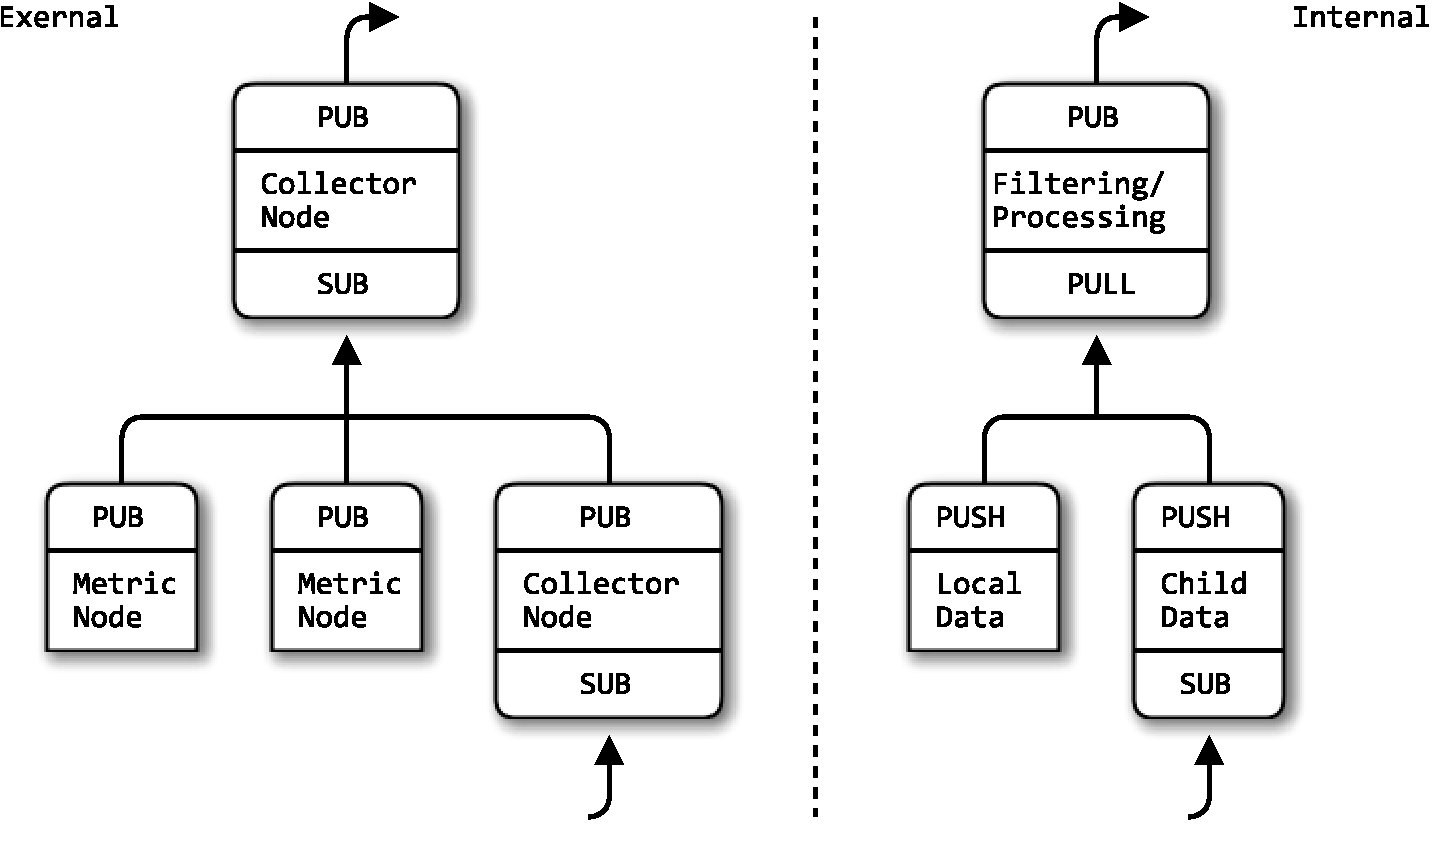
\includegraphics[scale=0.5]{data.pdf}
    \caption{Data Flow Diagram}
    \label{fig:proto_data_image}
\end{figure}

The \dcamp data flow protocol is very simple, comprised of a single data message type. The data flows from one node to
another via PUB/SUB sockets. Internally, data flows from the upstream data producers, through a filtering/processing
unit, and out to downstream data consumers via PUSH/PULL sockets.

When data rate is slower than a predefined threshold, heartbeats are sent instead to keep inter-node connections alive.

\begin{figure}[H]
\vspace{+10pt}
\begin{verbatim}
data-flow = *( METRIC / HUGZ )
\end{verbatim}
\vspace{-5pt}
\caption[Data Flow Specification]
	{Data Flow Specification: All messages are sent from child (Metric or Collector) to parent (Collector or Root).}
\label{fig:proto_data_spec}
\end{figure}

\subsubsection{Performance Measurement}

When discussing performance measurement, it is important to understand how metrics are sampled, calculated, and
presented to an end user.

Performance metrics, also called counters, are usually monotonically increasing values. That is, reading its raw,
instantaneous value is virtually meaningless; to correctly read the counter it must be sampled at two different points
in time and then calculated.

For example, when displaying a graph of data point for non-basic metric types, each data point is really a calculated
value of the value at the current timestamp and that at the previous timestamp. It is possible to look at fewer data
samples to first get a course-grain view (e.g. five-minute samples) of the metric before drilling in a looking at
finer-grain samples (e.g. one-second samples).

Non-monotonically increasing counters do exist (e.g. disk speed, Ethernet uplink speed, etc.), but these are usually
fairly static configuration values and do not need to be sampled frequently. \dcamp supports these types of counters
with the ``basic'' metric type.

Table \ref{tab:metric_types} shows how each of the \dcamp metric types are calculated. Note: unlike some other
performance measurement frameworks\cite{ganglia}, \dcamp stores all metrics in their raw, uncalculated form and only
presents a calculated value upon display.

\begin{table}
\begin{tabular}{|l|l|l|}
\hline
\textbf{Type} & \textbf{Contents of Single Sample} & \textbf{Calculation of Two Samples}
\\
\hline
basic & raw value at specified timestamp & \( C = V_{t_2} \)
\\
\hline
delta & raw value at specified timestamp & \( C = V_{t_2} - V_{t_1} \)
\\
\hline
rate & raw value at timestamp & \( C = (V_{t_2} - V_{t_1}) / (t_2 - t_1) \)
\\
\hline
average & raw value and raw base value at timestamp & \( C = (V_{t_2} - V_{t_1}) / (B_{t_2} - B_{t_1}) \)
\\
\hline
percent & raw value and raw base value at timestamp & \( C = ( (V_{t_2} - V_{t_1}) / (B_{t_2} - B_{t_1}) ) 100 \)
\\
\hline
\end{tabular}
\caption[Metric Types]
        {Metric Types: \(C\) represents the value calculated from two samples taken at \(t_1\) and \(t_2\). \(V\) is the
	 value and \(B\) is the base value in the \texttt{METRIC} message}
\label{tab:metric_types}
\end{table}

\subsubsection{Message Definitions}

\textbf{\texttt{METRIC}} is a five-frame message containing the performance metric data sampled by the Sensor service or
calculated by the Aggregation service. The \texttt{HUGZ} message is simply shorthand for \texttt{METRIC(type="HUGZ")}.

A single data sample MUST contain: source identifier (node or aggregation), metric identifier, timestamp, and one or two
values depending on the metric type.

In case of \texttt{HUGZ}, no other property strings are used, and Frames 3 through 5 are all empty. Frame 4 will be
non-empty for average and percent types.

NOTE: This message needs to be cleaned up...its a bit too verbose. I think just the config-seqid is needed to identify
      the metric being sampled.

\begin{figure}[H]
\vspace{+10pt}
\begin{verbatim}
Frame 0: data source (leaf or collector node address), as 0MQ string
Frame 1: properties, JSON-encoded as 0MQ string
Frame 2: time in ms epoch utc, 8 bytes in network order
Frame 3: value, 8 bytes in network order
Frame 4: base value, 8 bytes in network order; only for average and percent types

properties = *( type / detail / config / seqid )
type       = "type=" ( "HUGZ" / "basic" / "delta" / "rate" / "average" / "percent" )
detail     = "detail=" <string>
config     = "config-name=" <string>
seqid      = "config-seqid=" <integer>
\end{verbatim}
\vspace{-20pt}
\caption{\texttt{METRIC} Message Definition}
\label{fig:message_metric}
\end{figure}
